\section{PLC}
\frame{
	\ifdebug
	\frametitle{Outline\hfill{\color{red} \emph{M}}}
	\else
	\frametitle{Outline}
	\fi
	\tableofcontents[currentsection]
}

\subsection*{Algoritmo}
% Una subsection* crea un nuevo "grupo de puntos"

\frame{
	\ifdebug
	\frametitle{Algoritmo\hfill{\color{red} \emph{M}}}
	\else
	\frametitle{Algoritmo}
	\fi
	% Define block styles
\tikzstyle{decision} = [diamond, draw, fill=blue!20, 
    text width=4.5em, text badly centered, node distance=3cm, inner sep=0pt]
\tikzstyle{block} = [rectangle, draw, fill=blue!20, 
    text width=4em, text centered, rounded corners, minimum height=4em]
\tikzstyle{line} = [draw, -latex']

\tikzstyle{cloud} = [draw, ellipse,fill=red!20, node distance=3cm,
    minimum height=2em]
    
\begin{figure}[t]
\resizebox{0.9\textwidth}{!}{

\begin{tikzpicture}[node distance = 2cm, auto]
    % Place nodes
    \node [cloud] (init) {Tablero energizado};
    \node [block, below of=init] (run) {PLC run};
    \node [block, below of=run] (var) {Adq. Nivel y Caudal};
    \node [decision, below of=var](hhl){Nivel?};
    \node [block, below of=hhl](stop){Detener la planta};
    \node [decision, right of=hhl](hl){Nivel?};
    \node [block, below of=hl](alarm){Señal de alarma};
    \node [decision, right of=hl](set){Parám.?};
    \node [block, below of=set](param){Seteo de parámetros};
    \node [decision, right of=set](manual){Manual?};
    \node [block, below of=manual](control){Control manual};
    \node [block, right of=manual](on){Motores ON};
    \node [block, right of=on](state){Estado};
    \node [, below left of=stop](null){};
    %\node (null){};
%     % Draw edges
    \path [line,dashed] (init) -- (run);
    \path [line] (run) -- (var);
    \path [line] (var) -- (hhl);
    \path [line] (hhl) -- node {si} (stop) ;
    \path [line] (stop) |- (null);
    \path [line] (null) |- (run);%--++  (-3,0) |- (run);
    \path [line] (hhl) -- (hl);
    \path [line] (hl) -- node {si} (alarm);
    \path [line] (hl) -- (set);
    \path [line] (set) -- node {si} (param);
    \path [line] (set) -- (manual);
    \path [line] (manual) -- node {si} (control);
    \path [line] (manual) -- (on);
    \path [line] (on) -- (state);
    \path [line] (state) |- (null);
    \path [line] (alarm) |- (null);
    \path [line] (param) |- (null);
    \path [line] (control) |- (null);

\end{tikzpicture}
 }
\end{figure}

}

\frame{
	% Define block styles
\tikzstyle{decision} = [diamond, draw, fill=blue!20, 
    text width=4.5em, text badly centered, node distance=3cm, inner sep=0pt]
\tikzstyle{block} = [rectangle, draw, fill=blue!20, 
    text width=4em, text centered, node distance=3cm,rounded corners, minimum 
height=4em]
\tikzstyle{line} = [draw, -latex']

\tikzstyle{cloud} = [draw, ellipse,fill=red!20, node distance=3cm,
    minimum height=2em]
    
\begin{figure}[t]
\resizebox{0.745\textwidth}{!}{

\begin{tikzpicture}[node distance = 1.5cm, auto]
    % Place nodes
    \node [cloud] (init) {Tablero energizado};
    \node [block, below of=init] (init_param) {Inic. Parámetros};
    \node [block, below of=init_param] (run) {PLC run};
    \node [decision, right of=run](emer){Emerg?};
    \node [block, above of=emer] (set_emer) {Bandera Emergencia};
    \node [, right of=emer](null){};
    \node [block, right of=null,node distance = 1.5cm] (adq) {Adq. Nivel y 
Caudal};
    \node [decision, right of=adq](hhll){HHL LLL?};
    \node [block, above of=hhll] (set_hhll) {Error Nivel};
    \node [, right of=hhll](null_hhll){};
    \node [decision, right of=null_hhll,node distance = 1.5cm](hl){HL LL?};
    \node [block, above of=hl] (set_hl) {Alarma};
     \node [, right of=hl](null_hl){};
    \node [decision, right of=null_hl,node distance = 
1.5cm](set_param){Parám.?};
    \node [block, above of=set_param](param){Seteo de parámetros};
     \node [, right of=set_param](null_param){};
    
    \node [decision, below of=set_param](set_auto){Auto?};
    \node [decision, left of=set_auto](verif_band){Verifica Banderas?};
    \node [, below of=set_auto,node distance =3cm](null_auto){};
    \node [decision, below of=null_auto](band_emer){Ban emer?};
    \node [, below of=band_emer,node distance =4cm](null_band_emer){};

    
    \node  [block, below of=verif_band] (no_mot) {Parar Motores};
    \node  [block, left of=verif_band] (motores) {Motores};
    \node  [block, left of=motores] (pid) {Válv. PID};
    \node [, left of=pid](null_pid){};
    
    \node [decision, left of=band_emer](bomb1){Bomba 1?};
    \node [, left of=bomb1](null_bomb1){};
    \node [decision, left of=null_bomb1,node distance=1.5cm](bomb2){Bomba 2?};
    \node [, left of=bomb2](null_bomb2){};
    \node  [block, below of=bomb1] (set_bomb1) {Set Bomba 1};
    \node  [block, below of=bomb2] (set_bomb2) {Set Bomba 2};
    \node  [block, left of=null_bomb2,node distance = 1.5cm] (valv_manual) 
{Válv. Manual};
    
    \node [decision, left of=pid](enclav){Enclav?};
    \node [block, below of=enclav, node distance=4.5cm] (alarm_enclav) {Alarma 
Enclavamiento};
    
    
    
%     \node [block, below of=run] (var) {Adq. Nivel y Caudal};
%     \node [decision, below of=var](hhl){Nivel?};
%     \node [block, below of=hhl](stop){Detener la planta};
%     \node [decision, right of=hhl](hl){Nivel?};
%     \node [block, below of=hl](alarm){Señal de alarma};
%     \node [decision, right of=hl](set){Parám.?};
%     \node [block, below of=set](param){Seteo de parámetros};
%     \node [decision, right of=set](manual){Manual?};
%     \node [block, below of=manual](control){Control manual};
%     \node [block, right of=manual](on){Motores ON};
%     \node [block, right of=on](state){Estado};
%     \node [, below left of=stop](null){};
%     %\node (null){};
% %     % Draw edges

    \path [line,dashed] (init) -- (init_param);
    \path [line] (init_param) -- (run);
    \path [line] (run) -- (emer);
    \path [line] (emer) -- (set_emer);
    \path [line] (set_emer) -| (null);
    \path [line] (emer) -- (adq);
    \path [line] (adq) -- (hhll);
    \path [line] (hhll) -- (set_hhll);
    \path [line] (set_hhll) -| (null_hhll);
    \path [line] (hhll) -- (hl);
    \path [line] (hl) -- (set_hl);
    \path [line] (set_hl) -| (null_hl);
    \path [line] (hl) -- (set_param);
    \path [line] (set_param) -- (param);
    \path [line] (param) -| (null_param);
    \path [line] (set_param) -- (null_param);
    \path [line] (null_param) |- (set_auto);
    
    \path [line] (set_auto) -- (verif_band);
    \path [line] (set_auto) -- (band_emer);
 
    \path [line] (verif_band) -- (motores);
    \path [line] (verif_band) -- (no_mot);
    \path [line] (no_mot) -| (run);
    \path [line] (motores) -- (pid);
    
    \path [line] (band_emer) -- (bomb1);
    %\path [line] (band_emer) |- (set_bomb1);
    \path [line] (set_bomb1) -| (null_bomb1);
    \path [line] (bomb1) -- (set_bomb1);
    \path [line] (bomb1) -- (bomb2);
    \path [line] (set_bomb2) -| (null_bomb2);
    \path [line] (bomb2) -- (valv_manual);
    \path [line] (bomb2) -- (set_bomb2);
    
    \path [line] (pid) -- (enclav);
    \path [line] (valv_manual) -| (null_pid);
    \path [line] (enclav) -- (alarm_enclav);
    \path [line] (enclav) -| (run);
    \path [line] (alarm_enclav) -| (run);
    
    \path [line] (band_emer) -- (null_band_emer);
    \path [line] (null_band_emer) -| (run);
%     \path [line] (verif_band) -- (motores);
%     \path [line] (verif_band) -- (no_mot);
%     \path [line] (no_mot) -| (run);
%     \path [line] (motores) -- (pid);

%     \path [line] (set_param) -- (null_param);
%     \path [line] (set_param) -- (null_param);
%     \path [line] (set_param) -- (var);
%     \path [line] (run) -- (var);
%     \path [line] (run) -- (var);
    


%     \path [line,dashed] (init) -- (run);
%     \path [line] (run) -- (var);
%     \path [line] (var) -- (hhl);
%     \path [line] (hhl) -- node {si} (stop) ;
%     \path [line] (stop) |- (null);
%     \path [line] (null) |- (run);%--++  (-3,0) |- (run);
%     \path [line] (hhl) -- (hl);
%     \path [line] (hl) -- node {si} (alarm);
%     \path [line] (hl) -- (set);
%     \path [line] (set) -- node {si} (param);
%     \path [line] (set) -- (manual);
%     \path [line] (manual) -- node {si} (control);
%     \path [line] (manual) -- (on);
%     \path [line] (on) -- (state);
%     \path [line] (state) |- (null);
%     \path [line] (alarm) |- (null);
%     \path [line] (param) |- (null);
%     \path [line] (control) |- (null);

\end{tikzpicture}
 }
\end{figure}


}

\subsection*{Programacion}
\frame{
	\ifdebug
	\frametitle{Programación\hfill{\color{red} \emph{M}}}
	\else
	\frametitle{Programación}
	\fi
	\textbf{Lenguaje de Programación}

	\begin{itemize}
	 \item {\color{newcolor} Ladder:} lenguaje gráfico de programación.
	 \item {\color{newcolor} \textbf{Palabras} en memoria }
	\end{itemize}

\begin{table}[!t]
\tiny
\renewcommand{\arraystretch}{1.3}
\centering
\begin{tabular}{c||c||c}
\hline
\bfseries Tipo & \bfseries Word  & \bfseries Descripción\\
\hline \hline
Lect & MW2  & Lectura DP cell nivel \\
Lect & MW3  & Lectura DP cell caudal\\
Lect & MW4  & Valor Kp\\
Lect & MW5  & Valor Ti\\
Lect & MW6  & Valor Td\\
Lect & MW7  & Valor de lectura del SP \\
Lect & MW8  & Valor de lectura de la válvula \\
\hline
Esc & MW9 & Valor de escritura de la válvula (manual)\\
Esc & MW10  & Valor de escritura del SP \\
Esc & MW11  & Valor de escritura Kp \\
Esc & MW12  & Valor de escritura Ti \\
Esc & MW13  & Valor de escritura Td \\
\hline
\end{tabular}
\end{table}

}
\frame{
	\ifdebug
	\frametitle{Programación\hfill{\color{red} \emph{M}}}
	\else
	\frametitle{Programación}
	\fi

	\begin{itemize}
	 \item {\color{newcolor} \textbf{Banderas} en memoria}
	\end{itemize}
	\begin{table}[!t]
	\tiny
\renewcommand{\arraystretch}{1.3}
\centering
\begin{tabular}{c||c||c||c}
\hline
\bfseries Tipo & \bfseries Word & \bfseries Bit & \bfseries Descripción\\
\hline \hline
Lect & MW0 & X0 & Señal Run PLC\\
Lect & & X1 & Alarma HHL\\
Lect & & X2& Alarma LLL\\
Lect & & X3& Alarma HL\\
Lect & & X4& Alarma LL\\
Lect & & X5& Error en motores\\
Lect & & X6& Motor 1 encendido\\
Lect & & X7& Motor 2 encendido\\
Lect & & X8& Modo manual activado\\
Lect & & X9& Modo automático activado y funcionando\\
Lect & & X10& Planta funcionando sin errores\\
\hline
Esc & MW1 & X0& Switch Encender(1)/Apagar(0)\\
Esc & & X1& Manual(1)/Automático(0)\\
Esc & & X2& Cambiar parámetros PID\\
Esc & & X3& Cambiar Set Point\\
Esc & & X4& Manual(0)/Default(1)\\
Esc & & X5& Encender M1 (manual)\\
Esc & & X6& Encender M2 (manual)\\
Esc & & X7& Limpiar errores\\
Esc & & X8& Parada de emergencia\\
Esc & & X9& Limpiar señal de parada de emergencia\\
\hline
\end{tabular}

\end{table}

}

\subsection*{PID}
\frame{
	\ifdebug
	\frametitle{Controlador PID\hfill{\color{red} \emph{M}}}
	\else
	\frametitle{Controlador PID}
	\fi

	\textbf{Acción del controlador:}
	%{\color{newcolor} Acción de controlador}
	\begin{itemize}
	  \item Proporcional al error
	  \item Proporcional a la integral del error respecto del tiempo
	  \item Proporcional a la derivada del error respecto del tiempo
	 \end{itemize}

	 \vspace{0.5cm}
	{\color{newcolor} Método de Ziegler–Nichols - Sintonización}
	\begin{columns}
		\begin{column}{0.55\textwidth}
			\begin{center}
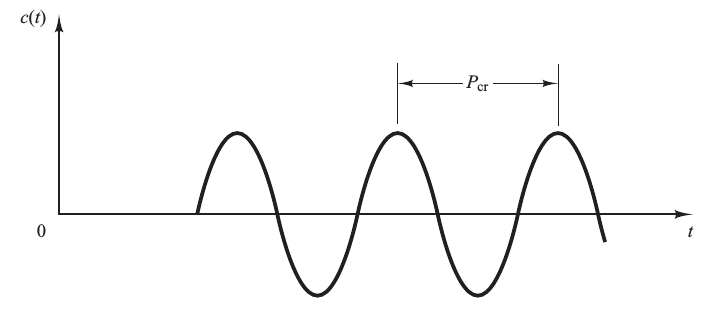
\includegraphics[width=\textwidth]{Sections/4-PLC/Images/segundometodo.png}
			\end{center}
		\end{column}
		\begin{column}{0.45\textwidth}
			\small
			\begin{table}[!t]
			\renewcommand{\arraystretch}{1.3}
			\centering
			\begin{tabular}{c||c||c}
			\hline
			\bfseries Kp  & \bfseries Ti & \bfseries Td\\
			\hline \hline
			 $0.6 \,Kp_{cr}  $ & $ 0.5 \, P_{cr}$ & $0.125 \, P_{cr} 
$\\
			\hline
			\end{tabular}
			\end{table}
		\end{column}

	\end{columns}
}

\frame{
	\ifdebug
	\frametitle{Sintonización PID\hfill{\color{red} \emph{M}}}
	\else
	\frametitle{Sintonización PID}
	\fi
	\textbf{Ganancias del controlador}
	%{\color{newcolor} Ganancias del controlador}

	\vspace{0.25cm}

	\begin{columns}
		\begin{column}{0.6\textwidth}
			\begin{center}
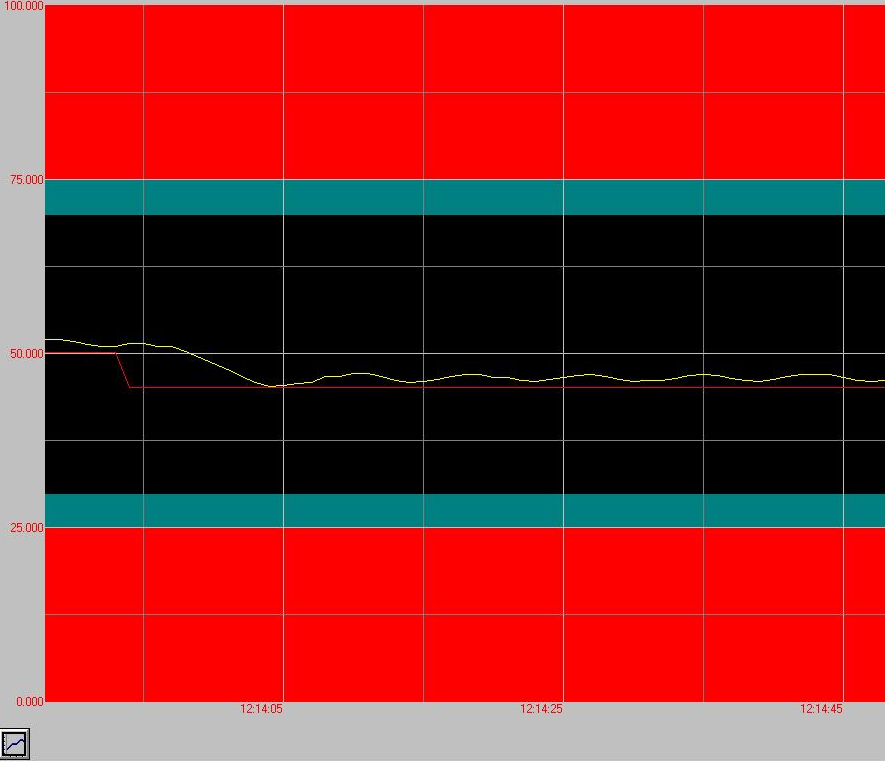
\includegraphics[width=\textwidth]{Sections/4-PLC/Images/oscperm.png}
			\end{center}
		\end{column}
		\begin{column}{0.4\textwidth}
			\begin{itemize}
			 \item {\color{newcolor2} Sin tiempo muerto:}
			    \begin{itemize}
			      \item $K_p $: $36$
			      \item $T_i $: $4$
			      \item $T_d $: $1$ 
			    \end{itemize}
			\end{itemize}
		\end{column}

	\end{columns}
}

\frame{
	\ifdebug
	\frametitle{Sintonización PID\hfill{\color{red} \emph{M}}}
	\else
	\frametitle{Sintonización PID}
	\fi
	\textbf{Ganancias del controlador}

	\vspace{0.25cm}

	%{\color{newcolor} Ganancias del controlador}
	\begin{columns}
		\begin{column}{0.6\textwidth}
			\begin{center}
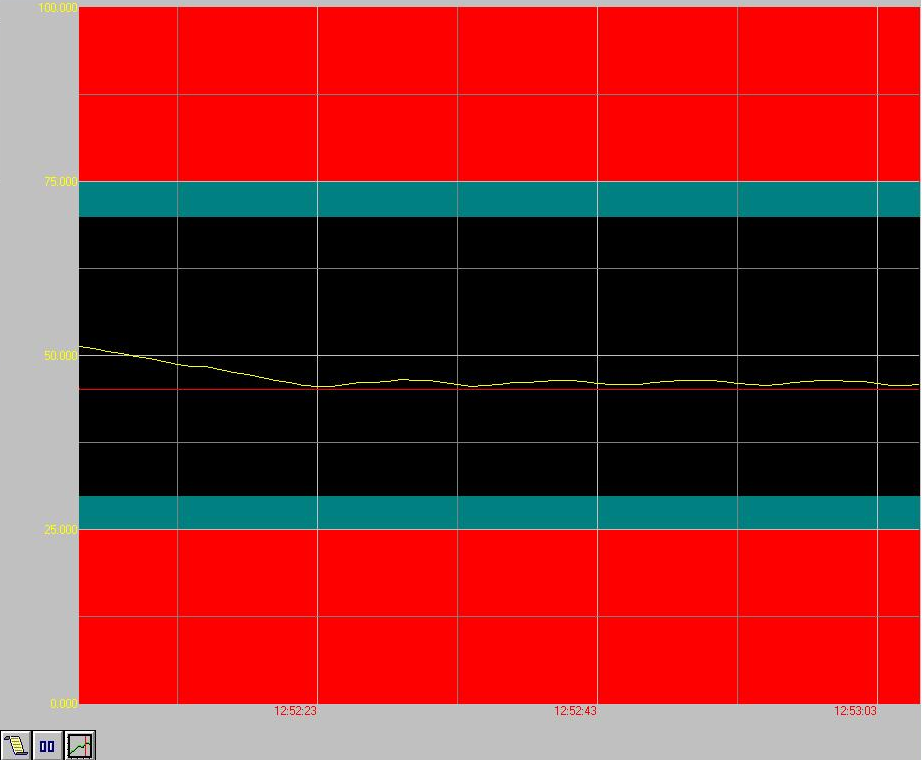
\includegraphics[width=\textwidth]{Sections/4-PLC/Images/oscpermtd.png}
			\end{center}
		\end{column}
		\begin{column}{0.4\textwidth}
			\begin{itemize}
			 \item {\color{newcolor2} Con tiempo muerto:}
			    \begin{itemize}
			      \item $K_p $: $72$
			      \item $T_i $: $5$
			      \item $T_d $: $1.25$ 
			    \end{itemize}
			\end{itemize}
		\end{column}
	\end{columns}
}
